\documentclass[10pt,conference,compsocconf]{IEEEtran}

\usepackage[hidelinks]{hyperref}
\usepackage{graphicx}

% Build: pdflatex report; bibtex report; pdflatex report; pdflatex report

\begin{document}
\title{Predicting Coronary Heart Disease from Survey Answers\\
with Gradient Boosting in NumPy}

\author{
  [Samuel Bachmann, Luca Civilla, Andrew Siminszky]\\
  \textit{CS-433 Machine Learning, EPFL, Switzerland}
}

\maketitle

\begin{abstract}
  We predict coronary heart disease (MICHD) from the answers of 328,135 people to
  the BRFSS 2015 survey, scored by the F1 of the positive class (8.8\% of the
  people). Decoding the survey codes with the official codebook, a
  gradient boosting written in NumPy and a decision threshold tuned for F1 reach a
  cross-validated F1 of $0.444 \pm 0.004$, 0.6 points above a regularized
  logistic regression, and 0.454 on the AIcrowd test set. One answer, asked only
  after a heart attack, reveals the label of 0.24\% of the people: we declare its
  use and measure it.
\end{abstract}

\section{Introduction}
Each of the 321 columns is an answer, a variable computed by the CDC from the
answers, or a field of the survey administration~\cite{brfss15}. Since only one
person in eleven is positive, predicting ``no'' for everyone gives an accuracy of
0.912 but finds nobody, so the metric is the F1 score, the harmonic mean of
precision and recall on the positive class. Our contributions are: (i) a decoding
of the answer codes, without which the logistic regression loses 1.3 points of
F1; (ii) a comparison of the six methods of the course on the same features;
(iii) a gradient boosting implemented from scratch, with a threshold chosen for
F1; (iv) an acceptance rule for changes fixed in advance, with the changes that
did not help and the one exception we made.

\section{Models and Methods}

\paragraph{Decoding}
The values are survey codes, not numbers: in \texttt{PHYSHLTH} (``days of poor
physical health'') 88 means none, 77 ``don't know'' and 99 ``refused''. We map
``don't know'', ``refused'' and ``not asked'' codes to missing values and ``none''
codes to 0, convert answers coded with a unit (``203'' means 3 times per week),
and re-number answers whose codes have no meaningful order (high blood pressure:
1 yes, 3 no, 4 borderline become 2, 0, 1). Many questions are asked only after a
given answer (skip patterns), so whether a value is missing carries information.

\paragraph{Inputs of the models}
The logistic regression and the course methods use 96 questions selected by hand
(43 secondary ones, e.g.\ on diet, vaccines or diabetes care), decoded by rules
written for them: 11 nominal answers are one-hot encoded with ``missing'' as a
level (levels with fewer than 200 rows dropped, the most frequent one as
reference), numeric answers are median-imputed with a missing indicator when at
least 10\% are missing, and all features are standardized and clipped to $\pm8$
($\approx$220 features). The gradient boosting reads 260 columns instead: all but
61 administrative (dates, sampling weights, phone screening) and redundant ones,
decoded with tables generated from the CDC codebook by one of us; missing values
get their own bin. All statistics are estimated on the training rows of each fold.

\paragraph{The HAREHAB1 answer}
The question HAREHAB1 (rehabilitation after a heart attack) is asked only to people
who reported a heart attack, in four states. It is answered in 773 training rows,
all positive, and in 238 test rows. It is part of the provided data, so we use it
(as an ``answered'' flag for the logistic regression, a bin for the trees), but a
real screening could not: without it the F1 of the logistic regression drops by
0.87 points (Table~\ref{tab:ablation}).

\paragraph{Course methods}
The six functions of \texttt{implementations.py} follow the course conventions:
the squared loss has a factor $1/2$, the logistic losses use labels in $\{0,1\}$,
and the regularized losses are returned without their penalty. Their
hyperparameters are in Table~\ref{tab:methods}. The regularized logistic
regression minimizes the summed log-loss plus $(\lambda_C/2)\|w\|^2$ with
$\lambda_C=10$, that is $\lambda = \lambda_C/(2N) \approx 1.9\cdot10^{-5}$ in the
convention of the course, for the $N$ rows of the training folds.

\paragraph{Final model}
Gradient boosting~\cite{friedman01} adds trees that each fit the gradient
$g=p-y$ and the curvature $h=p(1-p)$ of the log-loss at the current predictions
$p$. Each column is cut into at most 32 quantile bins plus a bin for missing
values, so a split is found by summing $g$ and $h$ per bin. Trees have depth 3;
each split also chooses the side of the missing values and keeps a sum of $h$ of
at least 5 per side; a leaf predicts $-\sum g/(\sum h + \lambda)$ with
$\lambda=10$. Each tree sees a random half of the rows and of the columns and is
shrunk by a rate of 0.05. The trees are fitted on 80\% of the training rows; the
other 20\% stop the boosting when their log-loss has not improved for 30 trees (at
most 1000) and set the threshold. On the full training set this gives 896 trees
and a threshold of probability 0.20.

\paragraph{Validation}
We use stratified 5-fold cross-validation (seed 42). In each fold everything is
fitted on the four training folds, including the threshold maximizing F1 (on the
training predictions for the linear models, on the 20\% validation rows for the
trees), and scored on the fifth. We report mean $\pm$ standard deviation over the
folds, and compare two variants by their paired difference per fold, in points
of F1 (pp). A change of the final model had to gain at least 0.30 pp, positive in
at least 4 of 5 folds, both on these folds and on new ones (seed 43). Rejected
variants (Table~\ref{tab:ablation}): an average with a neural network (64 ReLU
units), three boosting models stopped on different fifths (bagging), 64 bins,
depth 4, a rate of 0.025, and trees started from the logistic logits.

\section{Results}

\begin{table}[tbp]
  \centering\footnotesize\setlength{\tabcolsep}{4pt}
  \begin{tabular}{|l|l|c|}
    \hline
    Method & Hyperparameters & F1 \\
    \hline
    least squares & -- & 0.4237 $\pm$ 0.0029 \\
    ridge regression & $\lambda=10^{-5}$ & 0.4237 $\pm$ 0.0029 \\
    GD on MSE & 100 iter., $\gamma=0.9/L$ & 0.4223 $\pm$ 0.0029 \\
    SGD on MSE & $3N$ steps, $\gamma=2\cdot10^{-5}$ & 0.4211 $\pm$ 0.0031 \\
    logistic regression & 500 iter., $\gamma=1$ & 0.4384 $\pm$ 0.0038 \\
    reg.\ logistic regression & as above, $\lambda_C=10$ & 0.4384 $\pm$ 0.0038 \\
    \hline
    boosting, 96 questions & depth 3, rate 0.05 & 0.4424 $\pm$ 0.0049 \\
    boosting, 260 columns & same (final model) & 0.4440 $\pm$ 0.0043 \\
    \hline
  \end{tabular}
  \caption{F1 of the positive class, mean $\pm$ standard deviation over 5
    folds. The six course methods use the same $\approx$220 features; $L$ is the
    largest eigenvalue of $X^\top X/N$.}
  \label{tab:methods}
\end{table}

\begin{table}[tbp]
  \centering\footnotesize\setlength{\tabcolsep}{4pt}
  \begin{tabular}{|l|c|}
    \hline
    Change & $\Delta$F1 (pp) \\
    \hline
    \multicolumn{2}{|l|}{\textit{Logistic regression}} \\
    raw answer codes (no decoding) & $-1.28 \pm 0.16$ \\
    without the HAREHAB1 answer & $-0.87 \pm 0.12$ \\
    without the 43 secondary questions & $-0.48 \pm 0.21$ \\
    without the state & $-0.17 \pm 0.20$ \\
    without missing indicators & $-0.02 \pm 0.11$ \\
    $\lambda_C = 1$, $100$ & $-0.01$, $+0.03$ \\
    boosting on the same 96 questions & $+0.40 \pm 0.30$ / $+0.33$ \\
    \hline
    \multicolumn{2}{|l|}{\textit{Boosting on the 96 questions}} \\
    260 codebook columns (final model) & $+0.16 \pm 0.31$ / $+0.35$ \\
    average with a neural network & $+0.19 \pm 0.22$ / $+0.07$ \\
    bagging of 3 models & $+0.05$ \\
    64 bins, depth 4, rate 0.025 & $-0.14$, $-0.02$, $-0.15$ \\
    trees started from the logistic logits & $-0.15$ \\
    \hline
    \multicolumn{2}{|l|}{\textit{Final model}} \\
    threshold 0.5 instead of the F1-optimal one & $-19.0 \pm 0.7$ \\
    \hline
  \end{tabular}
  \caption{Ablation study: paired difference in F1 points with the model of each
    block, mean ($\pm$ std) over the 5 folds of seed 42, then mean over those of
    seed 43 after a slash; commas separate variants.}
  \label{tab:ablation}
\end{table}

\begin{figure}[tbp]
  \centering
  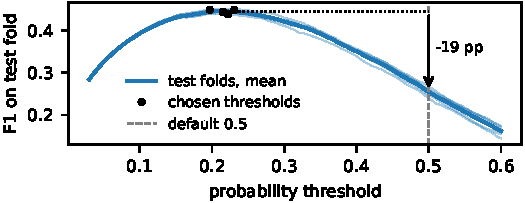
\includegraphics[width=0.92\columnwidth]{threshold}
  \caption{F1 of the final model on each test fold against the probability
    threshold; dots: thresholds chosen on the validation rows (20\% of the
    training folds).}
  \label{fig:threshold}
\end{figure}

Table~\ref{tab:methods} shows that the loss matters more than the optimizer: the
four squared-loss methods reach 0.421--0.424, the two logistic regressions 0.438
(gradient descent matches Newton's method within 0.01 pp).
Boosting adds 0.40 pp to
the logistic regression, positive on all 5 folds. Reading the 260 codebook
columns adds 0.16 pp on the folds of seed 42 (2 of 5 positive) and 0.35 pp on
those of seed 43 (5 of 5), so it fails our rule on the first folds. We made an
exception, after also seeing its AIcrowd score, because over the 10 folds its gain
(+0.26 pp, 7 positive) is twice that of the network average (+0.13 pp) and it
changes only the input of the same model. Table~\ref{tab:ablation} shows what
made the difference: decoding, the HAREHAB1 answer and the secondary questions,
then the model family; the other changes stay within the noise of the folds.
Fig.~\ref{fig:threshold} shows the largest single lever: the default threshold
0.5 flags too few people, while the F1-optimal one ($p \approx 0.2$, 13\% of each
test fold flagged) is close to the optimum of every fold.

The delivered submission (\texttt{python run.py}, 8.4 minutes on a laptop) scores
0.454 on AIcrowd (accuracy 0.875); the logistic regression scored 0.447 and the
boosting on 96 questions 0.452. The best online score of our team, 0.456, comes
from a heavier blend built by one of us: boosting of depth 6 on the same 260
columns (4 seeds, 70\%) and neural networks (10 seeds, 30\%), with 0.446 in its
own cross-validation (other folds, threshold tuned on the scored folds, hence
slightly optimistic). It runs for about an hour; we kept the simpler model.

\section{Discussion}
Once the data are decoded, the logistic regression and the boosting differ by
less than 0.7 points of F1, and the gains of the boosting and of the codebook
columns are of the order of the fold-to-fold noise (standard error about
0.2 pp~\cite{nadeau03}). The leaderboard moved with the cross-validation (0.447, 0.452, 0.454)
but sits about 0.9 points higher, and with about 9,700 expected positives its own
noise is about 0.4 pp. Precision stays low (0.38 in cross-validation, at a recall
of 0.54): a self-reported survey cannot separate many sick and healthy people,
and part of what the model ``predicts'' is a heart attack that people already
reported, through HAREHAB1.

\section{Summary}
Decoding, a gradient boosting written in NumPy and an F1-tuned threshold give an
F1 of 0.444 in cross-validation and 0.454 on the test set. \texttt{run.py}
reproduces the submission, \texttt{experiments.py} Tables~\ref{tab:methods}
and~\ref{tab:ablation} and Fig.~\ref{fig:threshold} (the rejected boosting
variants are on the branches \texttt{luca/ensemble} and \texttt{luca/levers}).

\bibliographystyle{IEEEtran}
\bibliography{literature}

\end{document}
